\section{Assignment 5}
	For this assignment, the year 2012 was utilized  in order to determine the ionospheric layers. The corresponding day of the year, Daily $F_{10.7}$, and Sunspot Number were 270, 139.9, and 84.5, respectively. The coordinating grid was kept the same as previous assignments. The figure below diplays the number density of various particles and ions as the altitude is varied. 

	\begin{figure}[h!]
		\centering
		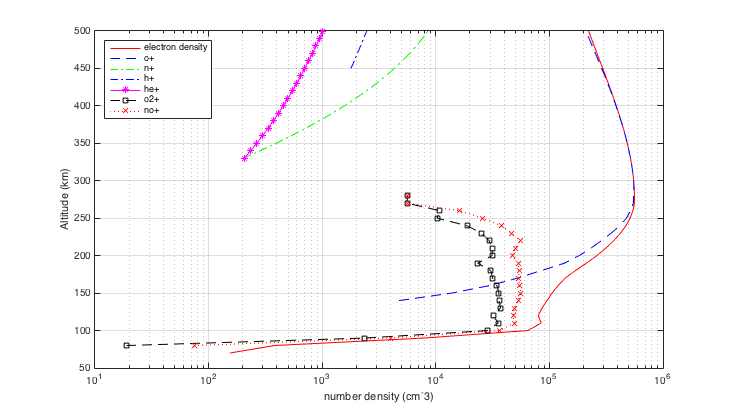
\includegraphics[scale=1.0]{images\ass5_properties_plot.png}
		\caption{Altitude vs. Particle Number Density ($cm^{-3})}
	\end{figure}

		\subsection{Discussion}
		Based on the densities shown in the particle density graph, it can be seen that D-layer exists between ~50-100 km. The presence of low amounts of NO ions corroborates the aforementioned statement as only a high-wavelength spectral line would be able to penetrate to this level and ionize the heavy ions. 
		\par
		The E-layer is somewhere between ~95-150 km. This layer consists of high amounts of $0_2^+$ and $N_2^+$ ions which are produced when x-rays and ultraviolet rays dissociate $O_2$ and $N_2$ molecules.
		\par
		The F layers is divided into the F1 and F2 layers. The F1 layer exists from between ~150-220 km. This can be determined by seeing the number density of electrons and $O^+$. Electron density is somewhere between $5e5$ to $5e6$ and $O^+$ density is higher due to the lighter particle floating to the higher regions. The F2 layer is between ~200-500 km. The lighter ions such as $He_+, N^+, and H^+$  exist in this layer due to their light weight.
		\par
		The Chapman layer differs from IRI model in displaying the number densities of particles especially in the F2 layer. These differences exist because the Chapman layer takes into account some parameters that the IRI model does not and vice versa. For example, the Chapman layer takes into account the Sun's zenith angle. In addition, the chapman layer method assumes that the radiation from sun is monochromatic, the atmosphere consists of only one gas, etc. These assumptions allow the chapman layer to create a "better density profile especially for the topside ionosphere (Jin)".


% References

% http://center.shao.ac.cn/geodesy/publications/Jin_2007EPS.pdf
% http://nova.stanford.edu/~vlf/IHY_Test/Tutorials/TheIonosphere/IonosphericMorphology.pdf
